\documentclass{beamer}

% select theme
\usetheme{CambridgeUS}
\usecolortheme{beaver}

\usepackage{kotex}
\usepackage{fancyvrb}
\usepackage{color}

% you need to generate pyg.tex by
% pygmentize -O full -f latex hello.c
\makeatletter
\def\PY@reset{\let\PY@it=\relax \let\PY@bf=\relax%
    \let\PY@ul=\relax \let\PY@tc=\relax%
    \let\PY@bc=\relax \let\PY@ff=\relax}
\def\PY@tok#1{\csname PY@tok@#1\endcsname}
\def\PY@toks#1+{\ifx\relax#1\empty\else%
    \PY@tok{#1}\expandafter\PY@toks\fi}
\def\PY@do#1{\PY@bc{\PY@tc{\PY@ul{%
    \PY@it{\PY@bf{\PY@ff{#1}}}}}}}
\def\PY#1#2{\PY@reset\PY@toks#1+\relax+\PY@do{#2}}

\def\PY@tok@gd{\def\PY@tc##1{\textcolor[rgb]{0.63,0.00,0.00}{##1}}}
\def\PY@tok@gu{\let\PY@bf=\textbf\def\PY@tc##1{\textcolor[rgb]{0.50,0.00,0.50}{##1}}}
\def\PY@tok@gt{\def\PY@tc##1{\textcolor[rgb]{0.00,0.25,0.82}{##1}}}
\def\PY@tok@gs{\let\PY@bf=\textbf}
\def\PY@tok@gr{\def\PY@tc##1{\textcolor[rgb]{1.00,0.00,0.00}{##1}}}
\def\PY@tok@cm{\let\PY@it=\textit\def\PY@tc##1{\textcolor[rgb]{0.25,0.50,0.50}{##1}}}
\def\PY@tok@vg{\def\PY@tc##1{\textcolor[rgb]{0.10,0.09,0.49}{##1}}}
\def\PY@tok@m{\def\PY@tc##1{\textcolor[rgb]{0.40,0.40,0.40}{##1}}}
\def\PY@tok@mh{\def\PY@tc##1{\textcolor[rgb]{0.40,0.40,0.40}{##1}}}
\def\PY@tok@go{\def\PY@tc##1{\textcolor[rgb]{0.50,0.50,0.50}{##1}}}
\def\PY@tok@ge{\let\PY@it=\textit}
\def\PY@tok@vc{\def\PY@tc##1{\textcolor[rgb]{0.10,0.09,0.49}{##1}}}
\def\PY@tok@il{\def\PY@tc##1{\textcolor[rgb]{0.40,0.40,0.40}{##1}}}
\def\PY@tok@cs{\let\PY@it=\textit\def\PY@tc##1{\textcolor[rgb]{0.25,0.50,0.50}{##1}}}
\def\PY@tok@cp{\def\PY@tc##1{\textcolor[rgb]{0.74,0.48,0.00}{##1}}}
\def\PY@tok@gi{\def\PY@tc##1{\textcolor[rgb]{0.00,0.63,0.00}{##1}}}
\def\PY@tok@gh{\let\PY@bf=\textbf\def\PY@tc##1{\textcolor[rgb]{0.00,0.00,0.50}{##1}}}
\def\PY@tok@ni{\let\PY@bf=\textbf\def\PY@tc##1{\textcolor[rgb]{0.60,0.60,0.60}{##1}}}
\def\PY@tok@nl{\def\PY@tc##1{\textcolor[rgb]{0.63,0.63,0.00}{##1}}}
\def\PY@tok@nn{\let\PY@bf=\textbf\def\PY@tc##1{\textcolor[rgb]{0.00,0.00,1.00}{##1}}}
\def\PY@tok@no{\def\PY@tc##1{\textcolor[rgb]{0.53,0.00,0.00}{##1}}}
\def\PY@tok@na{\def\PY@tc##1{\textcolor[rgb]{0.49,0.56,0.16}{##1}}}
\def\PY@tok@nb{\def\PY@tc##1{\textcolor[rgb]{0.00,0.50,0.00}{##1}}}
\def\PY@tok@nc{\let\PY@bf=\textbf\def\PY@tc##1{\textcolor[rgb]{0.00,0.00,1.00}{##1}}}
\def\PY@tok@nd{\def\PY@tc##1{\textcolor[rgb]{0.67,0.13,1.00}{##1}}}
\def\PY@tok@ne{\let\PY@bf=\textbf\def\PY@tc##1{\textcolor[rgb]{0.82,0.25,0.23}{##1}}}
\def\PY@tok@nf{\def\PY@tc##1{\textcolor[rgb]{0.00,0.00,1.00}{##1}}}
\def\PY@tok@si{\let\PY@bf=\textbf\def\PY@tc##1{\textcolor[rgb]{0.73,0.40,0.53}{##1}}}
\def\PY@tok@s2{\def\PY@tc##1{\textcolor[rgb]{0.73,0.13,0.13}{##1}}}
\def\PY@tok@vi{\def\PY@tc##1{\textcolor[rgb]{0.10,0.09,0.49}{##1}}}
\def\PY@tok@nt{\let\PY@bf=\textbf\def\PY@tc##1{\textcolor[rgb]{0.00,0.50,0.00}{##1}}}
\def\PY@tok@nv{\def\PY@tc##1{\textcolor[rgb]{0.10,0.09,0.49}{##1}}}
\def\PY@tok@s1{\def\PY@tc##1{\textcolor[rgb]{0.73,0.13,0.13}{##1}}}
\def\PY@tok@sh{\def\PY@tc##1{\textcolor[rgb]{0.73,0.13,0.13}{##1}}}
\def\PY@tok@sc{\def\PY@tc##1{\textcolor[rgb]{0.73,0.13,0.13}{##1}}}
\def\PY@tok@sx{\def\PY@tc##1{\textcolor[rgb]{0.00,0.50,0.00}{##1}}}
\def\PY@tok@bp{\def\PY@tc##1{\textcolor[rgb]{0.00,0.50,0.00}{##1}}}
\def\PY@tok@c1{\let\PY@it=\textit\def\PY@tc##1{\textcolor[rgb]{0.25,0.50,0.50}{##1}}}
\def\PY@tok@kc{\let\PY@bf=\textbf\def\PY@tc##1{\textcolor[rgb]{0.00,0.50,0.00}{##1}}}
\def\PY@tok@c{\let\PY@it=\textit\def\PY@tc##1{\textcolor[rgb]{0.25,0.50,0.50}{##1}}}
\def\PY@tok@mf{\def\PY@tc##1{\textcolor[rgb]{0.40,0.40,0.40}{##1}}}
\def\PY@tok@err{\def\PY@bc##1{\fcolorbox[rgb]{1.00,0.00,0.00}{1,1,1}{##1}}}
\def\PY@tok@kd{\let\PY@bf=\textbf\def\PY@tc##1{\textcolor[rgb]{0.00,0.50,0.00}{##1}}}
\def\PY@tok@ss{\def\PY@tc##1{\textcolor[rgb]{0.10,0.09,0.49}{##1}}}
\def\PY@tok@sr{\def\PY@tc##1{\textcolor[rgb]{0.73,0.40,0.53}{##1}}}
\def\PY@tok@mo{\def\PY@tc##1{\textcolor[rgb]{0.40,0.40,0.40}{##1}}}
\def\PY@tok@kn{\let\PY@bf=\textbf\def\PY@tc##1{\textcolor[rgb]{0.00,0.50,0.00}{##1}}}
\def\PY@tok@mi{\def\PY@tc##1{\textcolor[rgb]{0.40,0.40,0.40}{##1}}}
\def\PY@tok@gp{\let\PY@bf=\textbf\def\PY@tc##1{\textcolor[rgb]{0.00,0.00,0.50}{##1}}}
\def\PY@tok@o{\def\PY@tc##1{\textcolor[rgb]{0.40,0.40,0.40}{##1}}}
\def\PY@tok@kr{\let\PY@bf=\textbf\def\PY@tc##1{\textcolor[rgb]{0.00,0.50,0.00}{##1}}}
\def\PY@tok@s{\def\PY@tc##1{\textcolor[rgb]{0.73,0.13,0.13}{##1}}}
\def\PY@tok@kp{\def\PY@tc##1{\textcolor[rgb]{0.00,0.50,0.00}{##1}}}
\def\PY@tok@w{\def\PY@tc##1{\textcolor[rgb]{0.73,0.73,0.73}{##1}}}
\def\PY@tok@kt{\def\PY@tc##1{\textcolor[rgb]{0.69,0.00,0.25}{##1}}}
\def\PY@tok@ow{\let\PY@bf=\textbf\def\PY@tc##1{\textcolor[rgb]{0.67,0.13,1.00}{##1}}}
\def\PY@tok@sb{\def\PY@tc##1{\textcolor[rgb]{0.73,0.13,0.13}{##1}}}
\def\PY@tok@k{\let\PY@bf=\textbf\def\PY@tc##1{\textcolor[rgb]{0.00,0.50,0.00}{##1}}}
\def\PY@tok@se{\let\PY@bf=\textbf\def\PY@tc##1{\textcolor[rgb]{0.73,0.40,0.13}{##1}}}
\def\PY@tok@sd{\let\PY@it=\textit\def\PY@tc##1{\textcolor[rgb]{0.73,0.13,0.13}{##1}}}

\def\PYZbs{\char`\\}
\def\PYZus{\char`\_}
\def\PYZob{\char`\{}
\def\PYZcb{\char`\}}
\def\PYZca{\char`\^}
% for compatibility with earlier versions
\def\PYZat{@}
\def\PYZlb{[}
\def\PYZrb{]}
\makeatother





% syntax highlighted source code 넣는법:
% http://ubuntuforums.org/showthread.php?t=790610
% pygmentize 명령어가 실행될 수 있도록 하자.
% bash에 그냥 pygmentize라고 치면 어느 패키지를 설치해야 하는지 알려줌.
% then...
% 색깔 명령어가 define될 수 있도록... hello.c를 만든 다음,
% pygmentize -O full -f latex hello.c
% 를 돌리면 무엇을 include해야 하는지, define이 뭐가 필요한지 쭉
% stdout으로 출력해줌.
% pygmentize -f latex hello.c 로 나오는 verbatim문을 긁어붙이면 완성.
\begin{document}

% title slide
\begin{frame}
	\title{슬라이드 제목}
	\author{Force Core}
	\date{2010-05-06(목)}
	\titlepage
\end{frame}



% outline slide
\section*{Outline}
\begin{frame}
\tableofcontents
\end{frame}



\section{간단한 슬라이드}

\subsection{hello world!}

% 그냥 글자만 있는 슬라이드
\begin{frame}
	Hello World!
\end{frame}

% 제목도 들어갔다.
\begin{frame}
	\frametitle{제목도 넣기}
	이제 제목이 들어갔다.
	내용도 있음
\end{frame}

% 부제목이 있는 슬라이드
\begin{frame}
	\frametitle{제목도 넣기}
	\framesubtitle{부제목 넣었다}
	부제목을 넣은 슬라이드
\end{frame}

% with bullets
\begin{frame}
	\frametitle{Bullet이 있는 Slide}
	\begin{itemize}
		\item item1
		\item item2
		\item item3
	\end{itemize}
\end{frame}

\begin{frame}
	\frametitle{정의를 하는 슬라이드}
	\begin{definition}[영어 단어 Stream]
		\begin{itemize}
			\item Bach - 흐름, 내, 시내, 개울
			\item 유출, 분류
			\item 흐르다, 흘러가다, 흘러 나오다
			\item 잇달아 나오다, 끊임없이 게속되다
		\end{itemize}
	\end{definition}
\end{frame}

\begin{frame}
	\begin{figure}
	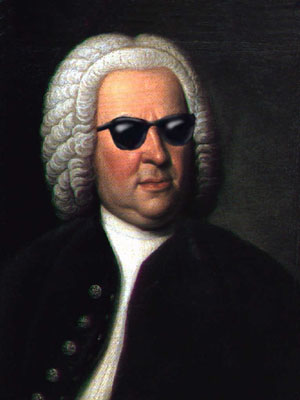
\includegraphics[width=0.3\columnwidth]{jpg/bach_shades.jpg}
	\end{figure}
	그림 넣은 슬라이드 \\
	``It's easy to play any musical instrument: all you have to do is touch the right key at the right time and the instrument will play itself.''
	\footnote{\url{http://thinkexist.com/quotation/it-s_easy_to_play_any_musical_instrument-all_you/13822.html}}
\end{frame}

\begin{frame}
	\frametitle{칼럼 넣은 슬라이드}
	\begin{columns}
	\begin{column}{0.5\textwidth}
		\begin{figure}
		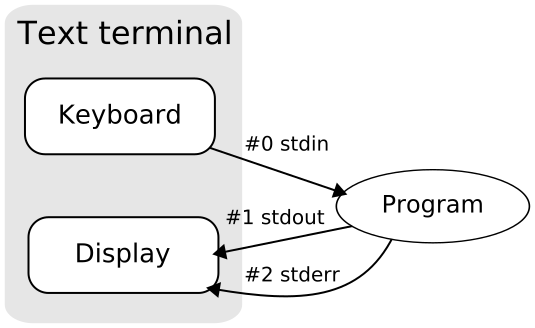
\includegraphics[width=0.9\columnwidth]{svg/Stdstreams-notitle}
		\end{figure}
	\end{column}

	\begin{column}{0.5\textwidth}
		\begin{itemize}
			\item stdout
			\item stderr
			\item stdin
		\end{itemize}
	\end{column}
	\end{columns}
\end{frame}

\begin{frame}[fragile] % Verbatim을 썼으므로 fragile표시를 해줘야 함.
	\frametitle{코드를 넣은 슬라이드}
	다음은 Hello World! 프로그램이다.
	c/pyg.sh hello.c 를 하면 나오는 내용을 여기 붙이면 되는 것임.

	\begin{Verbatim}[commandchars=\\\{\}]
\PY{c+cp}{#}\PY{c+cp}{include <stdio.h>}

\PY{k+kt}{int} \PY{n+nf}{main}\PY{p}{(}\PY{p}{)}
\PY{p}{\PYZob{}}
        \PY{n}{fprintf}\PY{p}{(} \PY{n}{stderr}\PY{p}{,} \PY{l+s}{"}\PY{l+s}{Program terminated with error!}\PY{l+s+se}{\PYZbs{}n}\PY{l+s}{"} \PY{p}{)}\PY{p}{;}
        \PY{k}{return} \PY{l+m+mi}{1}\PY{p}{;}
\PY{p}{\PYZcb{}}
\end{Verbatim}

\end{frame}

\subsection{서브섹션을 가르면 진도표에 반영됨}

\begin{frame}
	\frametitle{Caeser Cypher II}
	{\em \Large Practice1 - Caeser Cypher II}

	\vspace{5mm}
	중간 타이틀로서 나름 깔끔한듯.
	part기능에는 좀 어울리지 않아서 손으로 직접... 읔;;
\end{frame}

\section{다른 섹션}

\begin{frame}[containsverbatim]
	\frametitle{그냥 verbatim}
	터미널의 출력 따위
	\begin{verbatim}
	$ chmod -x a.out
	$ chmod +x a.out
	$ chmod -r test.c
	$ chmod +r test.c
	$ chmod -w test.c
	$ chmod +w test.c
	\end{verbatim}
\end{frame}

\subsection{Practice2 - chmod}

\begin{frame}
	\frametitle{Practice2 - chmod}
	{\em \Large Practice2 - chmod}

	\vspace{5mm}
	set, unset, get 함수를 완성하여 chmod를 따라해보자.
	set, unset, get함수에는 if문이 필요 없다.
\end{frame}



\end{document}

